%% ============================================================================
%% EchoPulse AI -- versión de envío a NALEF 2026 / CEUR-WS (clase ceurart)
%% Documento: system description paper, 5-8 páginas, en inglés.
%% Sin números de página ni encabezados: NO usar las opciones twocolumn ni hf.
%% Fuente: fusión de ECHOPULSE_CLEANED (documento base) + versión IEEE,
%% compactada para cumplir el límite de páginas. Versión larga: paper-largo.tex
%%
%% ---- DÓNDE ESTÁ EL PROYECTO ----
%% Este archivo vive dentro del fork local del estilo CEURART:
%%   ceurart/paper/paper.tex   (manuscrito)
%%   ceurart/tex/latex/ceurart/ceurart.cls  (clase generada, v0.6.2)
%%
%% ---- COMO COMPILAR ----
%%   bash build.sh            (compila paper.tex; usa LuaLaTeX si existe y si no,
%%                             el Tectonic portable de ../../tools/)
%%   bash build.sh paper-largo
%% La receta oficial de la clase es: lualatex x2 -> bibtex -> lualatex x3.
%% Sin numeros de pagina ni encabezados: no usar twocolumn ni hf.
%% ============================================================================
\documentclass[]{ceurart}

%% One can fix some overfulls
\sloppy
\usepackage{amsmath,amssymb,amsfonts}
\usepackage{graphicx}
\usepackage{textcomp}
\usepackage{url}
\usepackage{booktabs}
\usepackage{microtype}
\emergencystretch=1em

%% Buscar imágenes tanto en figures/ como en la raíz del proyecto.
\graphicspath{{figures/}{./}}

%% ---- notación matemática ----
\newcommand{\vect}[1]{\boldsymbol{#1}}
\newcommand{\mat}[1]{\mathbf{#1}}
\newcommand{\Real}{\mathbb{R}}
\newcommand{\softmax}{\operatorname{softmax}}
\newcommand{\LayerNorm}{\operatorname{LayerNorm}}
\newcommand{\cosine}{\operatorname{cos}}

\begin{document}

%% ---- nota de copyright exigida por la convocatoria (pie de la pág. 1) ----
\copyrightyear{2026}
\copyrightclause{Copyright for this paper by its authors.
  Use permitted under Creative Commons License Attribution 4.0
  International (CC BY 4.0). NALEF 2026, Cartagena, Colombia.}

%% ---- evento (CEUR-WS lo imprime en la primera página) ----
%% EDITOR: confirmar el nombre oficial del workshop/volumen CEUR-WS.
\conference{NALEF 2026: 9th Encuentro de Semilleros de Investigación,
  Cartagena, Colombia}

%% ---- título ----
\title{EchoPulse AI: A Hybrid Local Data Architecture for Multimodal Music
  Recommendation}
\subtitle{Integrating WASABI, MSD, Lyrics and TalkPlayData-2 Locally}

%% ---- autores ----
\author[1]{John Kennedy Landazuri Sandoval}[%
orcid=0009-0004-7437-2779,
email=john.landazuri@estudiante.fup.edu.co,
]
\cormark[1]

\author[1]{Cristian Camilo Ordoñez Quintero}[%
orcid=0000-0003-4157-1611,
email=camilo.ordonez@docente.fup.edu.co,
]
\cormark[2]

\author[2]{Hugo Armando Ordoñez Erazo}[%
orcid=0000-0002-3465-5617,
email=hugoordonez@unicauca.edu.co,
]

\author[1]{Cristian Méndez Rodríguez}[%
orcid=0000-0002-4489-2712,
email=cristian.mendez@docente.fup.edu.co,
]

\address[1]{IMS Research Group, Fundación Universitaria de Popayán,
  Popayán, Cauca, Colombia}
\address[2]{Research Group on Technology and Information Management (GT),
  Universidad del Cauca, Popayán, Cauca, Colombia}

\cortext[1]{Corresponding author.}
\cortext[2]{Corresponding author.}

%% ---- resumen ----
\begin{abstract}
Recommendation systems built on collaborative signals tend to keep surfacing
already popular tracks, because a song with no play history contributes little
evidence to the ranking. This paper presents EchoPulse AI, a locally deployed
multimodal recommender that addresses this visibility gap. The system processes
lyrical, acoustic, metadata and conversational data through a Triple-Encoder
Transformer, consolidating heterogeneous datasets (WASABI, Million Song
Dataset, Lyrics 1950--2019 and TalkPlayData-2) through a five-stage local
pipeline that runs without cloud dependencies. The methodology relies on a
curated Master Table of 5,710 tracks with complete multimodal coverage,
designed as a controlled proof of concept that isolates the cold-start problem.
Against collaborative filtering, BERT4Rec and SASRec baselines, EchoPulse AI
reaches competitive accuracy (Hit@10\,=\,0.312) while improving Intra-List
Diversity by 45.3\% and Emerging Artist Discovery by 157.9\%; core retrieval
components run below 250\,ms on consumer hardware. The current implementation
favours English-language content and is validated offline only, so scaling to
industrial catalogues and running online user studies are the key next steps.
\end{abstract}

%% ---- palabras clave ----
\begin{keywords}
Multimodal recommendation \sep
Transformer architecture \sep
Local data lakehouse \sep
Music information retrieval \sep
Cold-start problem \sep
Popularity bias mitigation
\end{keywords}

\maketitle

%% ============================================================================
\section{Introduction}
\label{sec:introduction}

Digital streaming reshaped the music business: global revenues hit USD 29.6
billion in 2024~\cite{ifpi2025report}. That expansion has not reached emerging
artists to the same degree. The first author played drums in bands across
Colombia for fourteen years, and the observation from inside those scenes is
consistent with the literature: new artists are rarely recommended.

Most platforms still lean heavily on collaborative filtering~\cite{ricci2015recommender}.
It performs well on high-volume catalogue and degrades on the cold
start~\cite{schein2002methods,adomavicius2005toward}: a new track receives no
exposure, gains no interactions, and is therefore excluded from the next
round of recommendations. In Latin American scenes the effect compounds,
because local artists compete for the same attention as global catalogue and,
increasingly, as generated background music.

Content-based approaches address this directly. Using lyrics, acoustic
properties and metadata makes it possible to rank what the music actually
sounds like~\cite{ricci2015recommender,aggarwal2016recommender}. The
Transformer~\cite{vaswani2017attention} maps long-range dependencies well, which
suits the structured, multi-layered nature of musical
content~\cite{baltruvsaitis2019multimodal}.

This paper introduces EchoPulse AI, a locally deployed multimodal recommender
built within the IMS Research Group at Fundación Universitaria de Popayán. The
deployment target was set by the conditions of the group rather than by
preference: a limited cloud budget and unreliable regional connectivity pushed
the design toward efficiency and reproducibility without cloud services. The
work contributes three things: a hybrid local data architecture that
consolidates heterogeneous music datasets through a five-stage pipeline; a
Triple-Encoder Transformer with specialised modules for lyrics, audio and
conversation; and an end-to-end evaluation on a controlled dataset showing that
diversity and emerging-artist visibility improve while retrieval accuracy stays
competitive with the baselines. Building the Master Table took more effort than
the modelling itself: reconciling incompatible identifier systems, imputing
missing values and aligning four datasets into one collection of 5,710 tracks
with complete multimodal coverage. That work shaped the architecture described
below.

Section~\ref{sec:framework} reviews the framework and hypotheses,
Section~\ref{sec:methodology} details the pipeline and model, and
Sections~\ref{sec:results}--\ref{sec:discussion} report the evaluation, its
scope and its limitations.

%% ============================================================================
\section{Framework and Hypotheses}
\label{sec:framework}

The Transformer self-attention mechanism~\cite{vaswani2017attention} computes
\begin{equation}
\text{Attention}(\mat{Q},\mat{K},\mat{V})
  = \softmax\left(\frac{\mat{Q}\mat{K}^\top}{\sqrt{d_k}}\right)\mat{V},
\label{eq:attention}
\end{equation}
letting the model weigh which parts of a sequence matter most. Songs are
organised in exactly that way, with verses, choruses and bridges recurring at a
distance, which is why sequence models transfer well to this material.
Multimodal machine learning formalises how to combine such heterogeneous
sources~\cite{baltruvsaitis2019multimodal}; cross-modal attention was effective
in vision-language models such as ViLBERT~\cite{lu2019vilbert} and
LXMERT~\cite{tan2019lxmert}, where early fusion is difficult to align across
heterogeneous feature spaces and late fusion leaves inter-modal correlations
unused. We adapt that mechanism to music. On the data side, the lakehouse
paradigm~\cite{armbrust2020delta} combines data-lake flexibility with
warehouse-style transactions; we implement the same requirements locally with
parquet-based storage, manual versioning and schema validation, which is what
supports reproducibility and traceability without cloud infrastructure.

Prior bias-mitigation work relies on post-processing re-ranking, inverse
propensity weighting or adversarial
debiasing~\cite{kaminskas2016diversity}, which adjust the output distribution
without giving cold-start items the content representation they lack. Sequential
baselines inherit the same flaw: BERT4Rec improves accuracy through
bidirectional encoding but keeps the popularity bias of its training
data~\cite{sun2019bert4rec}, and SASRec behaves likewise with
self-attention~\cite{kang2018self}. Conversational recommenders such as TalkPlay
generate recommendations in natural language but do not report a structured
multimodal fusion, and their generative components are not evaluated
quantitatively~\cite{choi2025talkplaydata2,gao2021advances}.

From this we posit two hypotheses. \textbf{H1 (contribution of multimodal
fusion):} fusing lyrical, acoustic and conversational modalities through
cross-attention improves retrieval quality and intent matching over baselines
that use interaction sequences or language alone, and each modality carries
information the others do not recover. \textbf{H2 (popularity bias mitigation):}
ranking by content affinity rather than by historical popularity increases
Intra-List Diversity (ILD) and Emerging Artist Discovery (EAD). Both are
expressed through a hybrid scoring function that combines semantic, acoustic
and lexical signals,
\begin{equation}
S(q,c) = \alpha \cdot \cosine(\vect{e}_q, \vect{e}_c)
       + \beta \cdot \left(1 - \frac{\|\vect{f}_q - \vect{f}_c\|_2}
       {\|\vect{f}_q\|_2 + \|\vect{f}_c\|_2}\right)
       + \gamma \cdot \frac{|T_q \cap T_c|}{|T_q \cup T_c|},
\label{eq:scoring}
\end{equation}
with $\alpha=0.4$ for semantic embeddings, $\beta=0.3$ for acoustic continuity
and $\gamma=0.3$ for lexical filtering by Jaccard similarity over token sets
$T_q$ and $T_c$. Equation~\eqref{eq:scoring} is the retrieval score; the final
ordering also applies the re-ranking blend described in
Section~\ref{sec:methodology}. A direct comparison against early- and
late-fusion variants is outside the present evaluation: H1 is tested against
interaction-only and language-only baselines and through the ablation in
Section~\ref{sec:results}.

%% ============================================================================
\section{Methodology}
\label{sec:methodology}

\subsection{Five-Stage Local Pipeline}
EchoPulse AI runs on a five-stage local architecture adapted from standard MLOps
practice for strictly local deployment. Figure~\ref{fig:architecture} traces the
flow from raw heterogeneous sources to local deployment, including the
evaluation feedback loop. The stages---Data Sources, Data Lake, Data Processing,
Data Modeling and Data Product---support reproducibility and traceability
through schema validation, directory-based snapshot isolation, hierarchical
$(\textit{year}, \textit{genre}, \textit{artist\_initial})$ partitioning and a
SQLite metadata catalog.

\begin{figure}
\centering
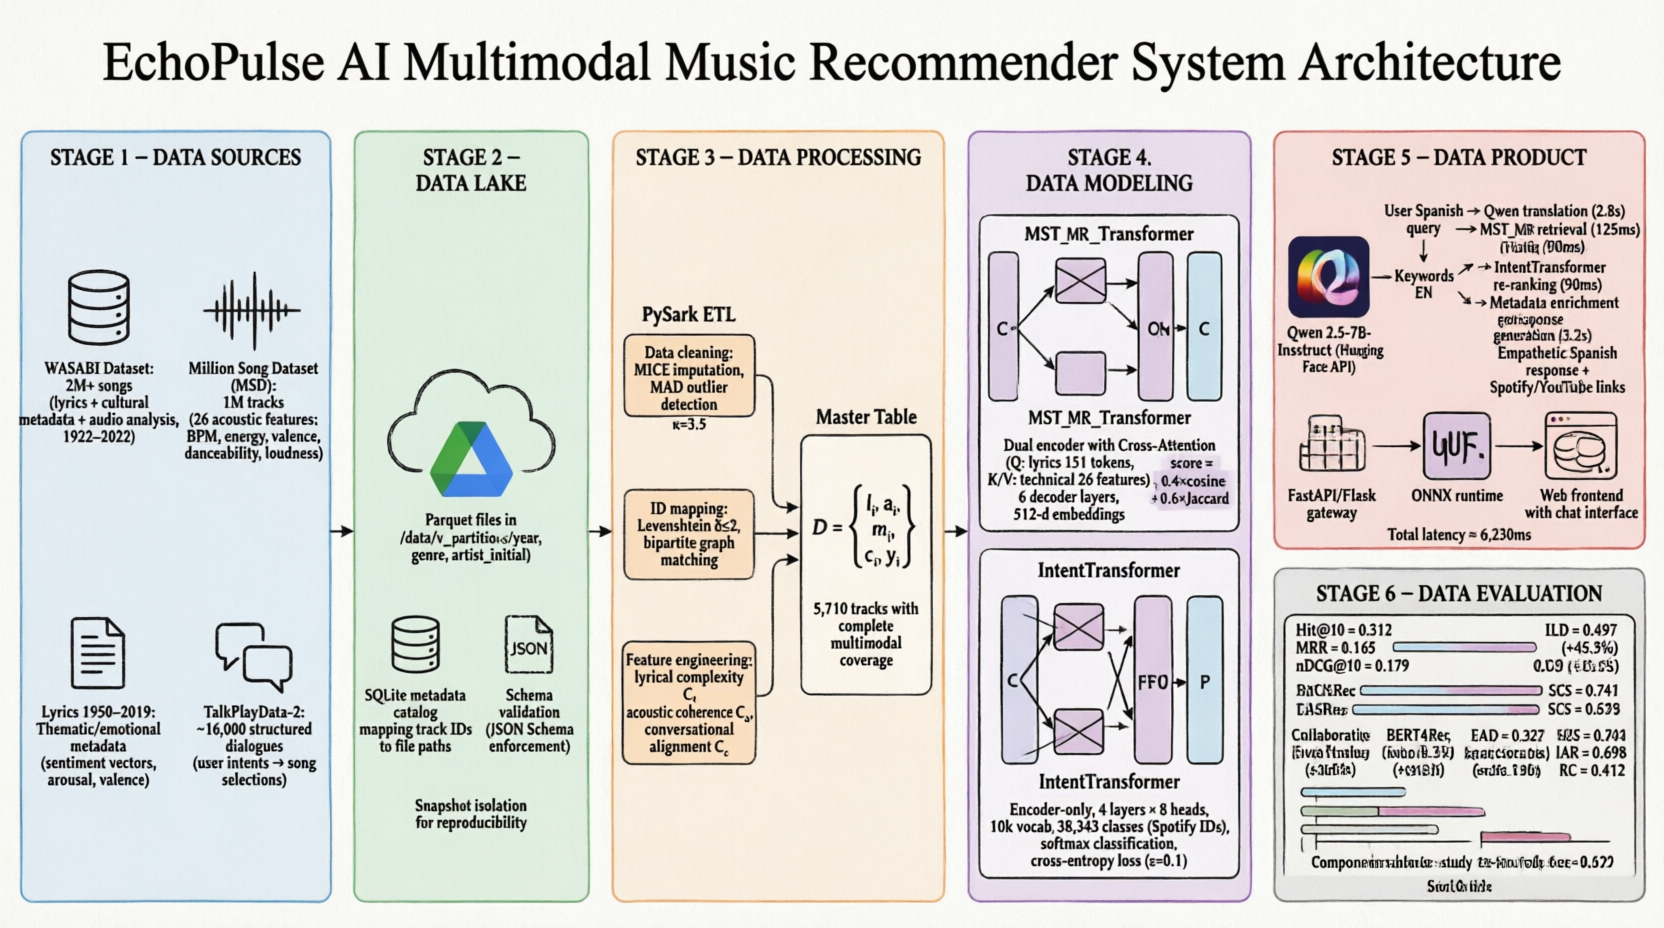
\includegraphics[width=0.55\textwidth]{archEchoPulse.png}
\caption{EchoPulse AI local data architecture: five-stage pipeline from
heterogeneous sources to local deployment, with an evaluation feedback loop.
Source: own elaboration.}
\label{fig:architecture}
\end{figure}

\subsection{Data Sources, Integration and Interaction Generation}
Four sources feed the system, each contributing a different modality: the WASABI
dataset for lyrics and cultural metadata~\cite{buffa2021wasabi}; the Million
Song Dataset (MSD) for 26 continuous acoustic features such as tempo, energy,
valence, danceability and loudness~\cite{bertin2011million}; Lyrics
1950--2019 for thematic and emotional metadata encoded as sentiment vectors
$\vect{s}\in\Real^{6}$~\cite{moura2020lyrics}; and TalkPlayData-2, a corpus of
about 16,000 structured dialogues that map user intentions to song
selections~\cite{choi2025talkplaydata2}.

Integration was the hardest step: MSD uses Echo Nest identifiers while WASABI
has its own system, so we matched records heuristically on the tuple
$(\textit{song\_name}, \textit{artist\_name}, \textit{release\_year})$ with a
Levenshtein distance threshold $\delta \leq 2$, reaching 84\% coverage with
validated acoustic vectors and complete lyrics. Missing values were handled by
MICE imputation~\cite{vanbuuren2011mice} and outliers flagged with the Median
Absolute Deviation at $\kappa=3.5$~\cite{leys2013mad}. The consolidated Master
Table is
\begin{equation}
\mathcal{D} = \{(\vect{l}_i, \vect{a}_i, \vect{m}_i, \vect{c}_i, y_i)\}_{i=1}^{N},
\qquad N = 5{,}710,
\label{eq:master}
\end{equation}
with tokenised lyrics $\vect{l}_i$, acoustic features
$\vect{a}_i \in \Real^{26}$, metadata embeddings $\vect{m}_i$, conversational
context $\vect{c}_i$ and target identifier $y_i$.

The 5,710-track table is a controlled proof of concept built to isolate the
effect of multimodal fusion on the cold-start problem. Deriving implicit
feedback for offline conversational evaluation is difficult, so we mapped the
structured TalkPlayData-2 dialogues onto the Master Table: intents expressed in
the dialogues were semantically matched to track embeddings, producing a
synthetic but structurally valid interaction matrix. The baselines
(collaborative filtering, BERT4Rec, SASRec) were trained on this identical
matrix with their official implementations and default hyperparameters. Two
consequences follow, and we record them as limits rather than as conveniences.
The matrix is itself generated by semantic matching in an embedding space, so a
model that consumes the same space begins with an advantage, which mainly
affects the conversational metrics; and a curated table of this size does not
represent the sparsity of an industrial catalogue.

\subsection{Triple-Encoder Transformer}
The first module, \textbf{IntentTransformer}, is an encoder-only Transformer
($L=4$ layers, $H=8$ heads, $d_{\text{model}}=256$) that encodes conversational
intent~\cite{wolf2020transformers}. It narrows the 38,343-track candidate set to
a top-10 for re-ranking, and is trained with cross-entropy and label smoothing
($\epsilon=0.1$)~\cite{mueller2019label}.

%% VERIFICAR (autores): las fuentes documentan L_l y el ancho de los encoders de
%% MST-MR de forma simbolica; faltan los valores numericos concretos.
The second module, \textbf{MST-MR} (Multimodal Sequence Transformer for Music
Recommendation), fuses modalities through cross-attention, following
principles from vision-language fusion~\cite{lu2019vilbert,tan2019lxmert}. A
lyrical encoder with $L_l$ transformer layers produces $\vect{h}_l$ from
tokenised lyrics, and a tabular MLP projects the 26 acoustic features into the
shared space as $\vect{h}_a$; each modality then attends to the other,
\begin{equation}
\text{CrossAttn}(\mat{Q}_l, \mat{K}_a, \mat{V}_a)
  = \softmax\left(\frac{\mat{Q}_l \mat{K}_a^\top}{\sqrt{d_k}}\right)\mat{V}_a,
\label{eq:crossattn}
\end{equation}
\begin{equation}
\vect{h}_{\text{fusion}}
  = \LayerNorm\bigl(\vect{h}_l + \text{CrossAttn}(\vect{h}_l, \vect{h}_a,
  \vect{h}_a)\bigr),
\label{eq:fusion}
\end{equation}
and the concatenation of $\vect{h}_{\text{fusion}}$ with the conversational
vector $\vect{h}_c$ is projected to a 512-dimensional song embedding $\vect{e}_s$
used in Equation~\eqref{eq:scoring}. The two weightings act at different stages: \eqref{eq:scoring} scores
candidates with $\alpha$, $\beta$ and $\gamma$, while the final ordering of the
surviving top-10 combines the neural similarity of $\vect{e}_s$ (40\%) with
lexical Jaccard similarity over the lyric tokens (60\%).

\subsection{Local Inference}
Serving uses a two-tier, CPU-optimised stack: a FastAPI gateway for validation,
orchestration and asynchronous response formatting, and an inference engine with
dynamic batching and INT8 quantization. In the throughput test that engine
reached 185 inferences per second against 73 for direct PyTorch serving, on a
different machine from the one used for training (an Intel Core i7-11800H)
~\cite{paszke2019pytorch,jacob2018quantization}. Quantisation cut the memory
footprint by 68\% at 1.2\% accuracy degradation. The deployment recorded a 98.4\%
request success rate, with fallback handling for cold starts, missing metadata
and API failures.

%% VERIFICAR (autores): protocolo de las pruebas de throughput y de tasa de
%% exito (tamano de lote, carga, duracion) y que maquina midio cada cifra.

%% ============================================================================
\section{Results and Demonstration}
\label{sec:results}

\subsection{Experimental Setup and Metrics}
Training and validation ran on a desktop machine with an
Intel\textsuperscript{\textregistered} Core\texttrademark{} i5-7200U CPU at
2.50\,GHz, 12.0\,GB of RAM and integrated Intel HD Graphics 620, i.e.\ commodity
consumer hardware. The model was trained on the Master Table with PyTorch 2.0
using CPU acceleration~\cite{paszke2019pytorch}, the AdamW optimizer at learning
rate $\eta=10^{-4}$~\cite{loshchilov2019decoupled}, batch size $B=32$ and early
stopping with patience $p=5$. Evaluation used a temporal 80\%/10\%/10\%
train/validation/test split to prevent data leakage.

We report retrieval quality and bias-mitigation quality. \textbf{Hit@K} is the
proportion of users with at least one relevant item in the top-$K$,
\begin{equation}
\text{Hit@K} = \frac{1}{|U|} \sum_{u \in U}
  \mathbb{I}\bigl(y_u \in \mathcal{R}_u^K\bigr);
\label{eq:hit}
\end{equation}
MRR captures the position of the first relevant item and nDCG@K weights relevant
items by position~\cite{jarvelin2002cumulated}. \textbf{Intra-List Diversity}
measures redundancy inside one list~\cite{ziegler2005improving},
\begin{equation}
\text{ILD} = \frac{2}{K(K-1)}\sum_{i<j} \bigl(1 -
  \cosine(\vect{e}_i, \vect{e}_j)\bigr),
\label{eq:ild}
\end{equation}
and \textbf{Emerging Artist Discovery} measures long-tail surfacing,
\begin{equation}
\text{EAD} = \frac{1}{K} \sum_{i=1}^{K}
  \mathbb{I}\bigl(\text{Listeners}(a_i) < \tau\bigr),
\qquad \tau = 10{,}000,
\label{eq:ead}
\end{equation}
where $\tau$ is the monthly-listener cut-off that separates long-tail from
catalogue artists, chosen before the experiments as the indicator closest to the
motivation of the work.

%% VERIFICAR (autores): falta indicar de que campo de los datos proceden los
%% recuentos de oyentes mensuales usados por tau. On the conversational side,
\textbf{SCS} measures alignment between the query and the recommended track with
BERT embeddings~\cite{devlin2019bert,gao2021advances},
\begin{equation}
\text{SCS} = \frac{1}{|U|}\sum_{u \in U}
  \cosine\bigl(\text{BERT}(q_u), \text{BERT}(m_{r_u})\bigr),
\label{eq:scs}
\end{equation}
\textbf{IAR} is the rate at which the top-1 result matches the explicit intent
stated in the dialogue, and \textbf{RC} is the BLEU-4 score of the generated
explanation against human-annotated references.

\subsection{Comparative Performance}
\begin{table}
\caption{Performance of EchoPulse AI against baselines on the shared interaction
matrix. Best results in bold.}
\label{tab:results}
\centering
\renewcommand{\arraystretch}{1.2}
\resizebox{\textwidth}{!}{%
\begin{tabular}{@{}lccccccc@{}}
\toprule
\textbf{Model} & \textbf{Hit@10} & \textbf{MRR} & \textbf{nDCG@10}
  & \textbf{ILD} & \textbf{EAD} & \textbf{SCS} & \textbf{IAR} \\
\midrule
Collaborative Filtering & 0.142 & 0.089 & 0.156 & 0.342 & 0.127 & 0.412 & 0.385 \\
BERT4Rec~\cite{sun2019bert4rec} & 0.158 & 0.095 & 0.172 & 0.389 & 0.145 & 0.438 & 0.401 \\
SASRec~\cite{kang2018self} & 0.164 & 0.102 & 0.178 & 0.412 & 0.168 & 0.451 & 0.423 \\
TalkPlay~\cite{choi2025talkplaydata2} & 0.189 & 0.118 & 0.165 & 0.445 & 0.201 & 0.623 & 0.587 \\
\textbf{EchoPulse AI} & \textbf{0.312} & \textbf{0.165} & \textbf{0.179}
  & \textbf{0.497} & \textbf{0.327} & \textbf{0.741} & \textbf{0.698} \\
\bottomrule
\end{tabular}}
\end{table}

\begin{figure}
\centering
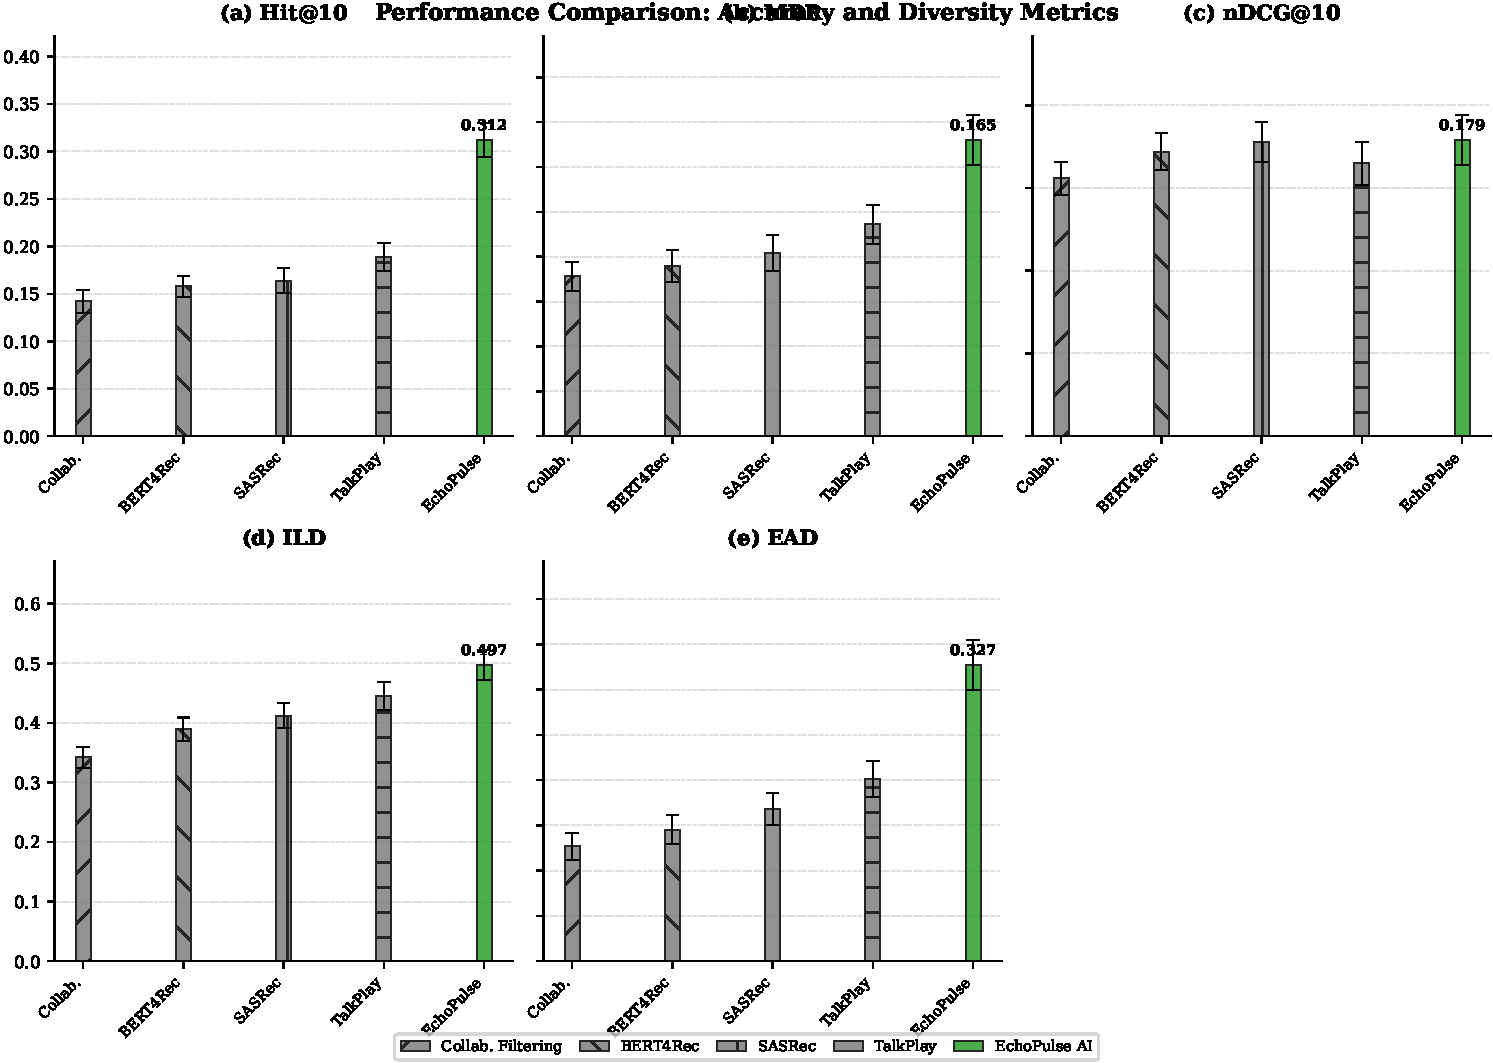
\includegraphics[width=0.55\textwidth]{fig1_performance_comparison.pdf}
\caption{Performance comparison across models for Hit@10, MRR, nDCG@10, ILD and
EAD. Error bars are 95\% confidence intervals from 5-fold cross-validation.
Source: own elaboration.}
\label{fig:performance}
\end{figure}

Table~\ref{tab:results} and Figure~\ref{fig:performance} are consistent with
both hypotheses. EchoPulse AI records twice the Hit@10 of the strongest
sequential baseline (0.312 vs.\ 0.164) and raises ILD by 45.3\% and EAD by
157.9\% relative to collaborative filtering. By popularity tier, the share of
emerging-artist recommendations goes from 12.7\% (collaborative filtering) and
20.1\% (TalkPlay) to 32.7\%, which is the distributional change the study was
designed to measure~\cite{brynjolfsson2011long,porcaro2021diversity}; the ILD
and EAD differences were tested with paired $t$-tests ($p<0.001$).

%% VERIFICAR (autores): unidad de contraste y n de los t-tests (usuarios,
%% queries o listas recomendadas).
The accuracy picture is not uniform across metrics: nDCG@10 nearly ties SASRec
(0.179 vs.\ 0.178), so the gain concentrates in top-of-list retrieval and in the
diversity indicators rather than in the complete ranking. Within this controlled
setting diversity improved without an accuracy penalty, but whether the same
holds on an uncurated catalogue remains open. The conversational metrics follow
the same pattern: SCS 0.741 against 0.623 and IAR 0.698 against 0.587 for
TalkPlay. RC applies only to systems that generate an explanation, so it is
reported for these two models alone: 0.412 BLEU-4 against 0.358.

The ablation study attributes the gains to specific components: removing the
IntentTransformer costs 7.9\% of MRR, eliminating MST-MR costs 15.2\% of Hit@10,
and cross-attention alone contributes 14.1\% of nDCG@10, which suggests that the
interaction between modalities, and not only the extra encoders, carries part of
the improvement. On latency, core retrieval takes 125\,ms,
re-ranking 90\,ms and metadata enrichment 15\,ms (215\,ms combined, mean of 100
runs), whereas the two Qwen 2.5 stages add 2,800\,ms for keyword translation and
3,200\,ms for the final response, giving an end-to-end pipeline of about 6.23\,s.

%% ============================================================================
\section{Discussion}
\label{sec:discussion}

Three points deserve comment. The ablation attributes a measurable share of the
gain to cross-attention, and each encoder removes work the others cannot
recover, which matches the multimodal literature~\cite{baltruvsaitis2019multimodal};
a direct early- versus late-fusion comparison is still missing. The local
lakehouse met the reproducibility and traceability targets without cloud
services, which is relevant for groups with limited budgets and unreliable
connectivity. The EAD result indicates that content-driven curation can
redistribute exposure inside a catalogue~\cite{brynjolfsson2011long}; for
musicians in secondary scenes such as Popayán, that is a practical difference
rather than a statistical one.

Relative to the baselines, the difference is architectural. BERT4Rec and SASRec
process interaction sequences only, so they inherit the popularity structure of
their training data; TalkPlay generates recommendations in language but does not
fuse modalities or evaluate its generative output. EchoPulse AI ranks by content
affinity, which is the only signal available for an artist without play history.

Limitations. The Master Table holds 5,710 tracks because the matching step
enforced complete multimodal coverage; this bounds the present study, even
though the fusion mechanism itself operates on fixed-dimensional latent spaces,
so inference cost grows linearly with catalogue size and approximate nearest
neighbour indexing (for example FAISS) is the expected route to an industrial
one. The system also mainly recommends English-language content, since WASABI,
MSD and TalkPlayData-2 are predominantly English, which limits its reach for
Spanish-language music and for regional Colombian genres such as vallenato,
cumbia and bambuco. The matching pipeline is specific to these four datasets, so
adapting it to arbitrary catalogues needs more flexible ingestion and automated
schema mapping. The $\sim$6\,s end-to-end latency, driven by the LLM stages,
rules out latency-sensitive uses until caching or distillation is added.
Finally, the evaluation is offline: it measures ranking and generation quality on
synthetic interactions rather than on real users, so no claim about satisfaction
or long-term listening is supported yet.

%% ============================================================================
\section{Conclusions}
\label{sec:conclusion}

We presented EchoPulse AI, a locally deployed multimodal music recommender that
consolidates heterogeneous datasets through a five-stage local pipeline and fuses
lyrical, acoustic, metadata and conversational signals with cross-attention, so
that content affinity rather than historical popularity drives the ranking. On a
controlled 5,710-track Master Table it improved Intra-List Diversity by 45.3\%
and Emerging Artist Discovery by 157.9\% over collaborative filtering, while
keeping accuracy competitive (Hit@10\,=\,0.312) and recording the best SCS, IAR
and RC among the compared systems. Those figures come from synthetic
interactions and offline evaluation; the next measurement has to come from real
listeners. The Master Table construction and the interaction-generation scripts
will be released so that the pipeline can be reproduced.

%% VERIFICAR (autores): confirmar donde se publicaran esos scripts antes de
%% afirmar la disponibilidad.
Future work runs in four directions: scaling to industrial-size catalogues with
ANN indexing while preserving multimodal integrity; controlled online studies
that measure perceived quality and diversity satisfaction; multilingual
adaptation to Spanish lyrics and Latin American genres with encoders such as
mBERT or XLM-R; and a reinforcement-learning loop from human feedback that
updates cross-attention weights from user corrections, together with
per-modality encoders and distillation for edge deployment.

%% ============================================================================
\begin{acknowledgments}
This work was supported by the IMS Research Group at Fundación Universitaria de
Popayán. The authors declare no competing interests relevant to the content of
this article.
\end{acknowledgments}

%% ============================================================================
%% Declaración obligatoria sobre IA generativa (política CEUR-WS, enero 2025).
%% EDITOR: ajustar herramientas y actividades a lo realmente realizado.
\section*{Declaration on Generative AI}
During the preparation of this work, the author(s) used generative AI tools in
order to: check grammar and spelling, and reformulate prose. After using these
tool(s)/service(s), the author(s) reviewed and edited the content as needed and
take(s) full responsibility for the publication's content.

%% ============================================================================
\bibliography{sample-ceur}

\end{document}
